% tk_kappa_rate: effective rate against successful recalls (DIAGRAMS.md item 25); lambda = 1.5
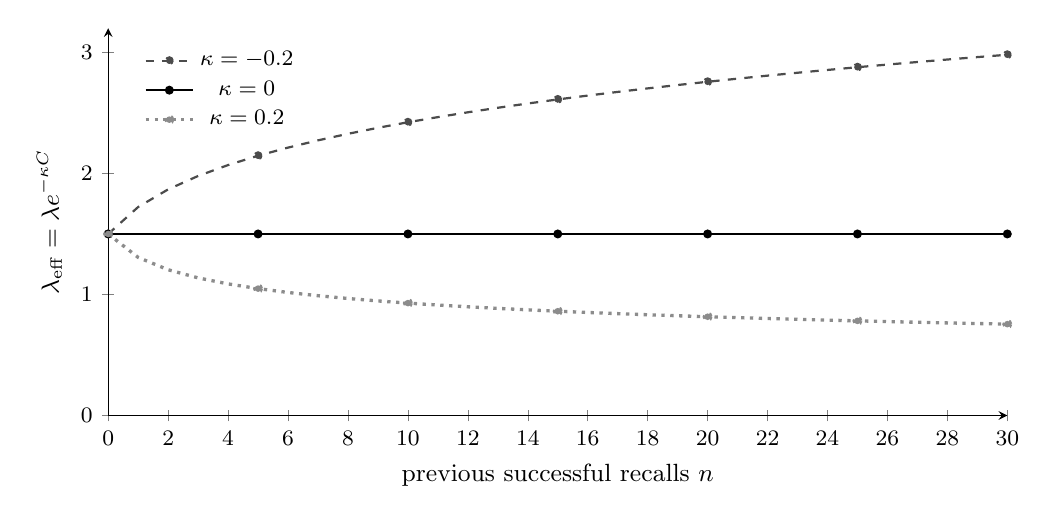
\begin{tikzpicture}
  \begin{axis}[width=13cm, height=6.5cm, xmin=0, xmax=30, ymin=0, ymax=3.2,
    xlabel={previous successful recalls $n$}, ylabel={$\lambda_{\mathrm{eff}}=\lambda e^{-\kappa C}$}, axis lines=left,
    legend pos=north west, legend style={font=\footnotesize, draw=none, fill=none},
    label style={font=\small}, tick label style={font=\footnotesize}]
    % C = log(1 + n); n = 0..30 (integer samples)
    \addplot[black!70, thick, dashed, mark=*, mark size=1.2pt, mark repeat=5, domain=0:30, samples=31] {1.5*exp(0.2*ln(1+x))};
    \addlegendentry{$\kappa=-0.2$}
    \addplot[black, thick, mark=*, mark size=1.2pt, mark repeat=5, domain=0:30, samples=31] {1.5*exp(0*ln(1+x))};
    \addlegendentry{$\kappa=0$}
    \addplot[black!45, very thick, dotted, mark=*, mark size=1.2pt, mark repeat=5, domain=0:30, samples=31] {1.5*exp(-0.2*ln(1+x))};
    \addlegendentry{$\kappa=0.2$}
  \end{axis}
\end{tikzpicture}
